\subsection{UPPLÄGG}
\label{Upplagg}

\begin{figure}[htb!]\centering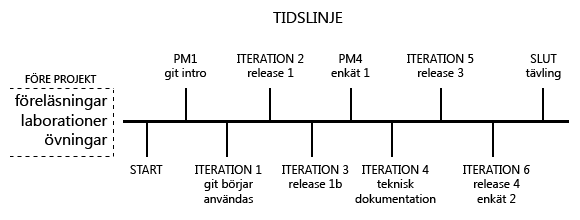
\includegraphics[width=0.75\textwidth]{Tidslinje.png}\caption{Visar tidsupplägget i projektet med viktiga händelser (PM = Planeringsmöte)}\label{fig:Timeline}\end{figure}

Vi lade upp arbete så att vi inte skulle lägga för mycket fokus på att använda Git som VCS då det är mycket ny information. Vårt team som vi skulle utbilda har inte varit i någon kontakt med Git innan men har inte heller några djuprotade arbetsätt med något annat versionhanteringssystem. Vi har delat upp upplägget för gruppen i tre faser. Första fasen är rent teoretisk och vi försöker hålla den på så grundläggande nivå som möjligt. Vi måste ständigt hålla i åtanke att för de flesta i gruppen som vi introducerar Git till har aldrig arbetat med något projekt innan av denna storlek. Vilket innebär att de har fullt upp med mycket annat och ger vi dem för mycket teori så kommer den ändå inte befästas. Gruppen har redan en god insikt till vikten av att kunna arbeta parallellt och vill lära sig mer om det. 

Då vi också var nya till Git bara någon månad tidigare så förstår vi deras situation och har lättare för att skriva ner en kort guide på de mest nödvändigaste kommandona för att kunna arbeta med vårt projekt [Appendix A]. Denna guide delar vi ut på första planeringsmötet så alla kan direkt komma igång med att klona ner och arbeta med koden på första långlabben. Vi tilldelar även en i gruppen att läsa på mer teori och även testa lite själv, på så vis har de en VCS expert inom gruppen då det kan kännas lättare att prata med varandra.
 
Fas två uppstår vid första labben och för det flesta är därmed deras mer teoretiska lärande färdigt. Här efter kommer de uteslutande lära sig av vad de ser och gör. Det vill säga att de ser vilka fördelar Git har och i vilka situationer man använder sig av olika funktioner. I fas två är gruppen fortfarande väldigt outbildad vilket leder till att vi coacher går runt och hjälper dem vid mer komplicerade kommandon och händelser. Till att börja med så behöver de inte lära sig dessa alls utan bara kunna det som gavs till dem i fas ett. Allt efter som så får de själva skriva in kommandona och vi står bakom och instruerar och bara kontrollerar så att allt görs rätt. Vissa i gruppen som inte vill lära sig så mycket om Git kommer stanna i denna fas.

Efter några veckor av labbande kommer fler och fler i gruppen att ta till sig arbets sättet och inte tillkalla oss då de redan vet vilka kommandon som ska skrivas. De är då som fas tre inleds med mycket mer självgående användande utav Git. De vet själva vad som ska göras och kommer själva med förslag när de vill brancha för att till exempel arbeta i tätt samarbete med en annan grupp för att uppnå ett bättre resultat snabbare. För sådana strukturella beslut som att det går snabbare att två grupper branchar ut och arbetar tillsammans godkänner vi det först, men inte för att de inte tekniskt klarar det utan att vi fortfarande kan utvärdera om det finns någon vinning i att göra det.

Det är för det mesta väldigt säkert att låta grupperna själva experimentera själva så fort de har lärt sig grunderna eftersom Git är väldigt robust och man kan nästan alltid återskapa det mesta.

Detta speciellt då vi har minst fem stycken lokala repon med komplett historik samt en server. Följer de även den utdelade guiden och commitar ofta upp till sina egna lokala repon så kan man återställa nästan alla fel.

\subsection{PLANERINGSMÖTEN}

I slutet av varje långlabb ska studenterna skriva ett par meningar om den specifika XP practice som de har fokuserat på. Vi har även lagt till att de också ska skriva om saker och ting som går bra och mindre bra med gruppen och vårt arbete, där vi belyst att om det är några problem med Git så ska de gärna ta upp dem här då vi coacher lättare kan ta tag och åtgärda dem. Dessa punkter tas sedan upp på våra schemalagda planeringsmöten för diskussion och reflektion. Vi kommer här med förslag till lösningar på hur vi ska åtgärda dessa och om någon i gruppen har något sätt. Här ser vi om vi till exempel skulle behöva skriva en ytterligare guide för att sätta in gruppen i de lite svårare funktionerna eller om de kan lära sig dem som beskrivet ovan i \ref{Upplagg} 

I slutet av planeringsmötena delar vi ut spikes till studenterna och om det har varit något som flera har uppfattat som svårt eller problematiskt inom Git så sprider vi kunskapen genom att någon gör ett grundligare undersökning varför det blev så och hur vi ska göra i fortsättningen. För det absolut mesta så vet vi coacher redan detta men  vi trycker hårt på att teamet ska besitta all kunskap själva och inte vara beroende utav oss coacher. Det kan även förekomma flera tillfällen då gruppen tycker att det är lättare eller smidigare att fråga varandra istället för oss coacher.

Det är viktigt att vi alla i gruppen också ska kunna ha tillgång till koden hemma för att kunna göra eventuella spikes så som till exempel kod granskning eller undersöka förslag till hur det är bäst att vidare utveckla en viss gren av programmet. För att detta ska fungera så har vi skrivit ihop en kort guide på den gemensamma trac-hemsidan. Där har vi också lagt upp ett shell-script som konfigurerar Git till deras inställningar utan att studenterna själva behöver skriva några kommandon.

Under de senare veckorna då gruppen arbetar mer självständigt med Git så skapar vi brancher även för de spikes som kräver något ur repot men även ska uppdatera repot till en ny version. Ledningen av kursen har beslutat att det får inte skrivas någon kod som trycks upp i repot mellan långlabbarna men gruppen får till exempel uppdatera JavaDoc eller teknisk dokumentation Det är viktigt för oss att dessa spikes inte blir för många och att de inte jobbar direkt på vår huvudbranch (master) utan att vi innan långlabben börjar kan merga ihop brancherna. Dessa merges ska alltid gå automatiskt då det inte ska vara flera brancher med samma ändringar. Till exempel så kan vi en vecka ha en spike med JavaDoc uppdateringar och en spike med att uppdatera manualen. Dessa två blir brancher för att kunna arbeta hemifrån utan att störa folk som vill ladda ner koden och få en halvt färdig skriven JavaDoc eller manual. Direkt då långlabben startar tar man en utav brancherna och mergar ihop den med master. Detta blir i git endast en fast forward och inga merge konflikter då det är bara en person som har ändrat. Sedan går vi till den andra spiken och gör det samma. Git löser denna merge-konflikten automatiskt då den tekniska dokumentationen inte har gjort några ändringar i några Java-filer och JavaDocen inte ska ha gjort några ändringar i den tekniska dokumentationen.

Ledningen för kursen har även godkänt att större refaktoriseringar utav hela programmet arkitekt kan vara bra att göra hemma då det förövrigt är produktionsstop då det annars skulle bli väldigt stora och svåra merge konflikter. När vi har dessa spikes är det viktigt att den spikegruppen är den ända som arbetar med koden och att alla har en god förståelse på vilka ändringar som kommer att göras och hur systemet kommer att se ut efteråt. Det är viktigt att lägga detta arbete på en egen branch då arbetet kan göras stegvis med flera commits under tiden. Att göra refaktoriseringar stegvis är inte bara bra för att andra får lättare att integrera sin kod utan att man lättare själv kan gå tillbaka om något inte blir bra. En annan mycket viktig aspekt på varför refaktoriseringen inte får ske på huvudbranchen är om den inte skulle lyckas bli klar så ska det inte vara några problem och alla kan bara arbeta på som vanligt. Skulle refaktoriseringen sedan bli klar någon timme in under labben så kan man fortfarande merga ihop den då. Det medför dock att man måste vara noggrann med den funktionaliteten som har tillkommit under tiden.

\subsection{GIT KONFIGURATION}

Git är mycket fritt och kan användas på många olika sätt där ingen är bunden att ställa sig i en hierarki. Vi har dock valt att arbeta med Git på ett lättförståligt sätt där alla hämtar(pull) det senaste från en server. På detta vis löser vi det krångliga som kan uppstå med att hämta från flera håll. Alternativet skulle vara att när en grupp har blivit klar med en story så hämtar alla ner hans version och mergar ihop med sitt eget. Här blir det dock lite rörigt i vår situation då vi enligt XP anda gör par byten och det slutar snabbt med att man inte har någon aning om vilken dator och inloggning man sitter på. Ett annat vanligt sätt att arbeta på är att ha en så kallad Gatekeeper~\cite{Gatekeeper} som alla hämtar ifrån. När ett par av utvecklare är färdiga med en story så säger man till Gate keepern som då hämtar från deras, kontrollerar ändringarna och kanske testkör programmet. När han är nöjd säger han till alla att det finns en ny version hos honom som alla ska hämta. Detta sättet är för visso mer säkert och röd kod sprider sig inte när någon har gjort fel. Dock så tycker vi coacher att detta inte känns så agilt och den snabbheten som är så viktig går lite förlorad. Det betyder även att teamet är beroende av denna enda “bättre vetande” personen som skall granska alla arbeten, vilket vi inte heller tycker går helt enligt XP. Vi vill med vår grupp uppnå en väldigt självgående sammansättning där vi coacher inte ska ha någon avgörande roll, och vi vill även att gruppen ska fungera vi eventuella bortfall. 
Vi har därför valt det upplägget som vi har och delar istället ut en task på att något annat utvecklingspar granskar en story innan den anses helt färdig. 


\subsection{UNDERSÖKNINGAR}

För att mer konkret kunna analysera vår utvekling och ge oss feedback om hur bra matrialet och vår undervisning är så har vi lämnat ut en enkät [Appendix B]. I enkäten försöker vi adressera de olika faserna och se hur framgångsrika de har varit. Vi har ställt enkla frågor för att se hur lätt det var att ta till sig teorin i fas ett. Att komma igång med ett naturligt arbetsflöde i fas två. Vi undersöker huruvida de känner sig bekväma med Git och får djupare försåelse för det genom terminalen i steg tre, samt hurvida de skulle kunna tänka sig att arbeta med det i framtiden för en eventuellt fas fyra. Vi ger ut enkäten två gånger under kursens gång för att kunna analysera några förändringar. Den första gången är efter cirka halva tiden då de flesta i gruppen är i mitten eller slutet av fas två och den andra gången vi undersöker är på sista mötet då allt arbete med Git ska vara avklarat. 